\mysection{User Interface Design}
In this section we will show some mockups in order to describe Travlendar+ user navigation.

\mysubsection{Login \& User Profile}
The login interface is composed by email and password fields. After the insertion of the credentials the user will be able to access to his calendar and personal page.
\begin{figure}[H]
	\centering
	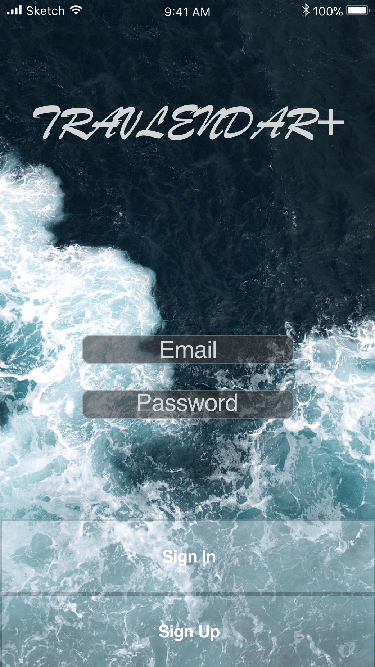
\includegraphics[scale=0.23]{Images/Interface/Login/1_login_form}
	\hspace{0.5cm}
	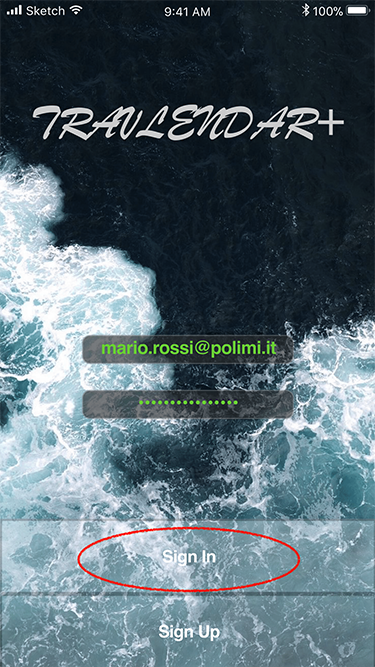
\includegraphics[scale=0.23]{Images/Interface/Login/2_login_form_filled}
	\hspace{0.5cm}
	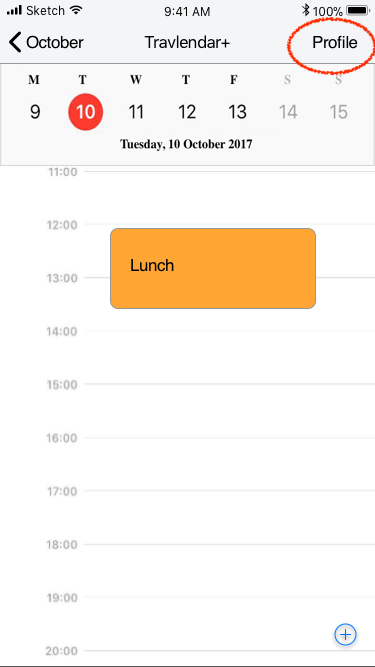
\includegraphics[scale=0.23]{Images/Interface/Login/3_calendar+lunch}
	\hspace{0.5cm}
	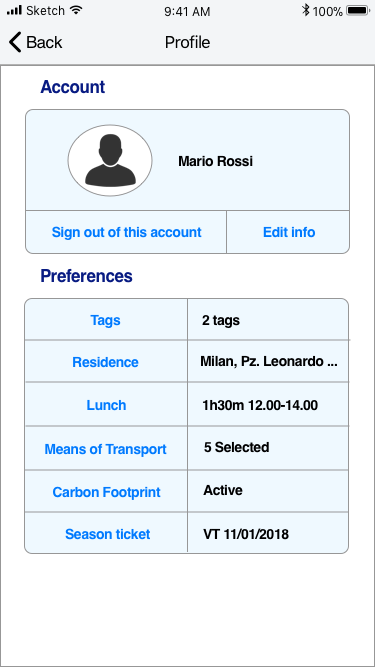
\includegraphics[scale=0.23]{Images/Interface/Login/4_profile_no_trips}
	\caption{Login Sketches}
\end{figure}

\mysubsection{Add Event}
By tapping on the add button on the bottom-right side of the screen it’ll be possible to plan a trip or add an event.
\begin{figure}[H]
	\centering
	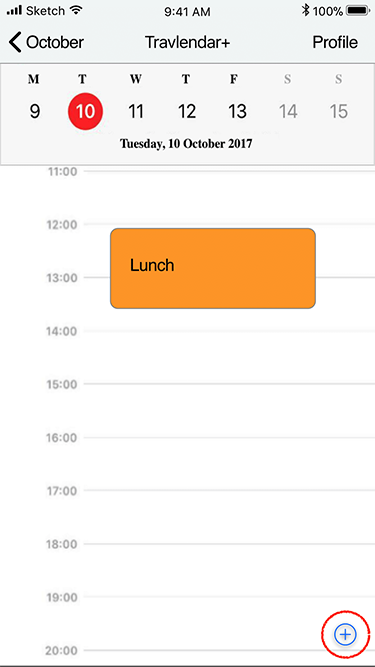
\includegraphics[scale=0.23]{Images/Interface/Calendar/1_calendar+lunch}
	\hspace{0.5cm}
	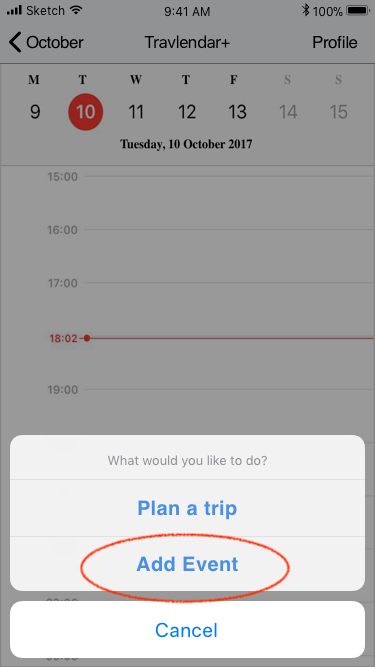
\includegraphics[scale=0.23]{Images/Interface/Calendar/2_add_menu}
	\hspace{0.5cm}
	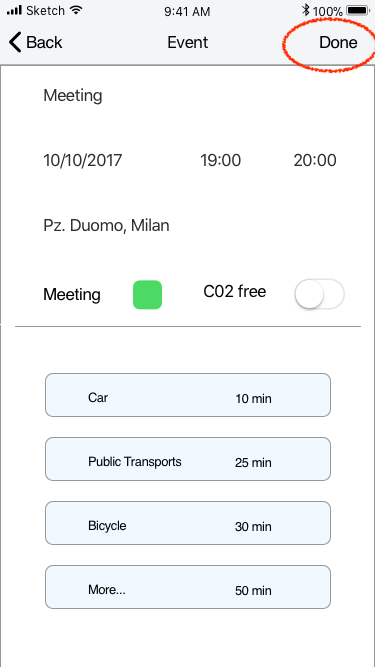
\includegraphics[scale=0.23]{Images/Interface/Calendar/3_single_event_view}
	\hspace{0.5cm}
	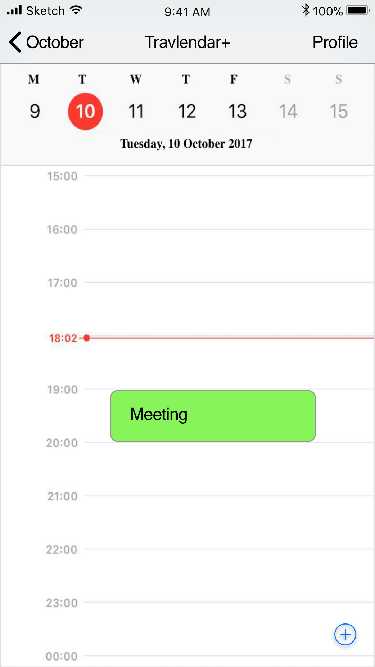
\includegraphics[scale=0.23]{Images/Interface/Calendar/4_calendar+meeting}
	\caption{Add Event Sketches}
\end{figure}

\newpage
\mysubsection{Lunch}
An everyday lunch event is created by default at the beginning of the time window indicated by the user. Furthermore, during the creation of an event, the system will move the lunch break and/or shrink its duration if needed.
\begin{figure}[H]
	\centering
	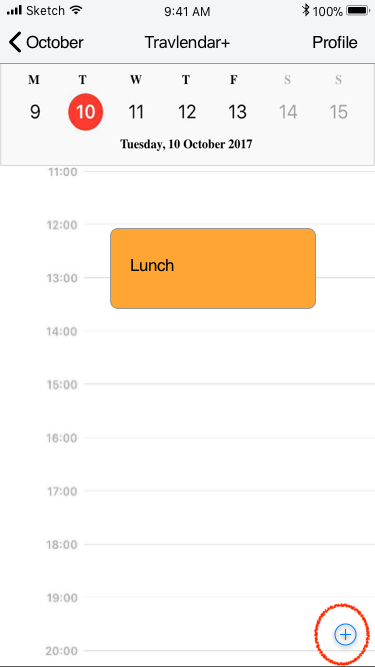
\includegraphics[scale=0.23]{Images/Interface/Lunch/1_calendar+lunch}
	\hspace{0.5cm}
	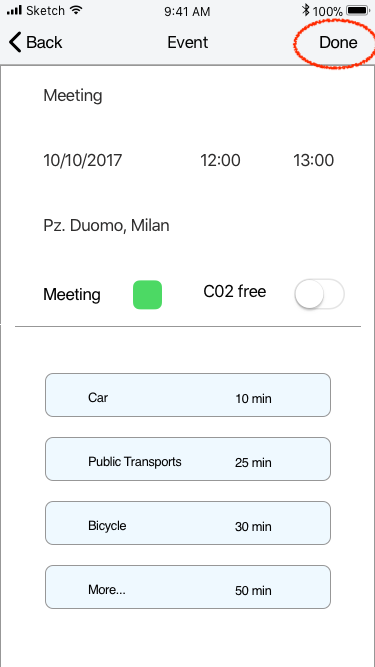
\includegraphics[scale=0.23]{Images/Interface/Lunch/2_single_event_view}
	\hspace{0.5cm}
	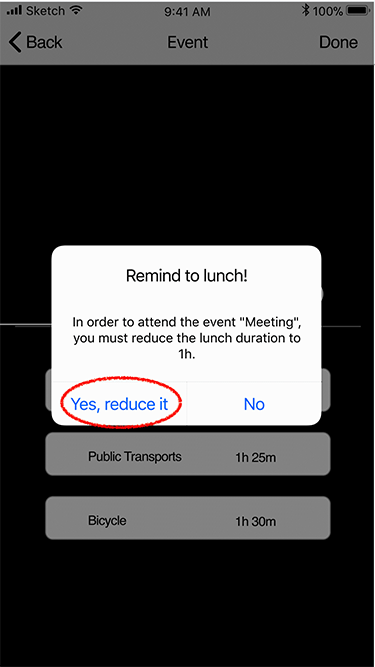
\includegraphics[scale=0.23]{Images/Interface/Lunch/3_lunch_warning}
	\hspace{0.5cm}
	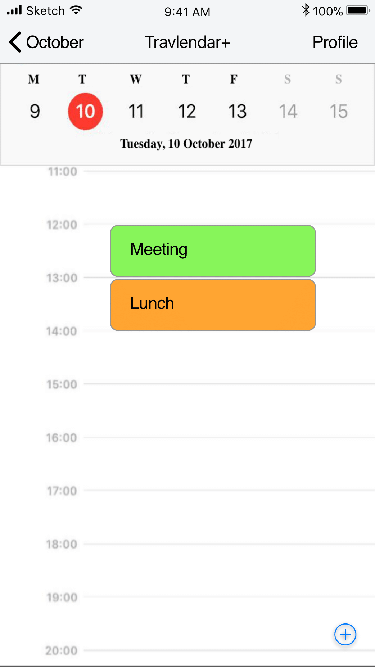
\includegraphics[scale=0.23]{Images/Interface/Lunch/4_calendar+meeting+lunch}
	\caption{Lunch Sketches}
\end{figure}

\mysubsection{CO$_2$ free}
It can be enabled or disabled as show below.
\begin{figure}[H]
	\centering
	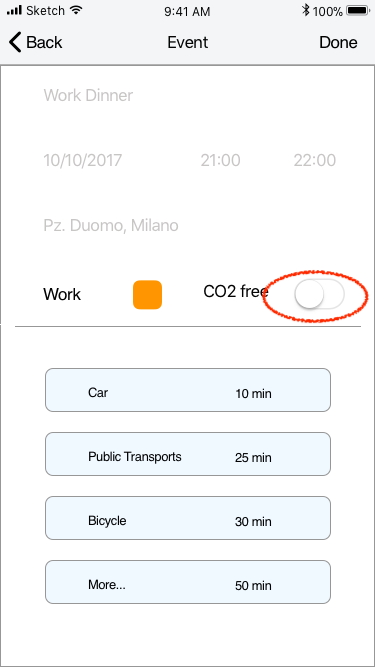
\includegraphics[scale=0.23]{Images/Interface/CO2/1_C02_disabled}
	\hspace{0.5cm}
	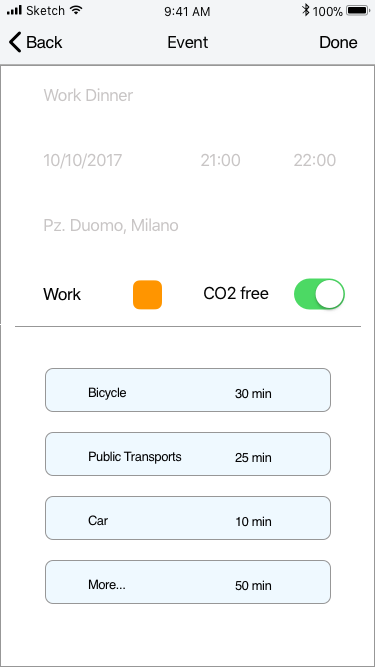
\includegraphics[scale=0.23]{Images/Interface/CO2/2_CO2_enabled}
	\caption{CO$_2$ Sketches}
\end{figure}

\newpage
\mysubsection{Weather Forecast}
A blue arrow will connect two reachable events. If the arrow is yellow, it means that the weather forecast is not optimal.
\begin{figure}[H]
	\centering
	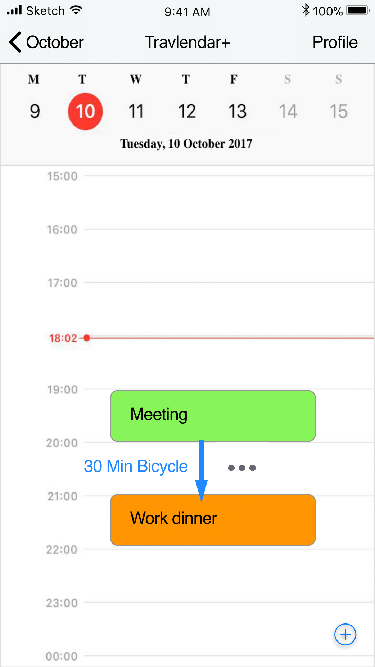
\includegraphics[scale=0.23]{Images/Interface/Weather_Forecast/1_optimal}
	\hspace{0.5cm}
	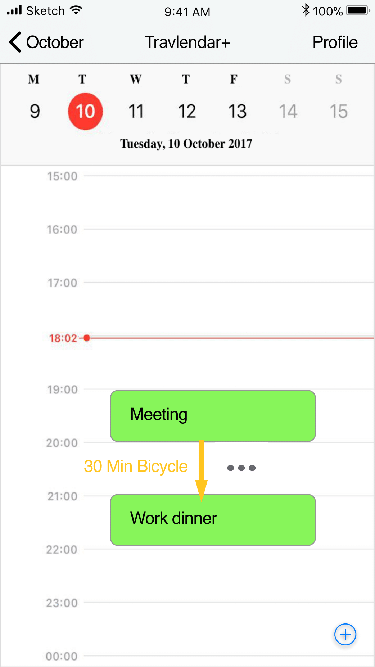
\includegraphics[scale=0.23]{Images/Interface/Weather_Forecast/2_rain}
	\caption{Weather Forecast Sketches}
\end{figure}

\mysubsection{Directions}
By tapping on the event its details will be shown.
By tapping on one item of the means list (the bottom side of picture 2) reported below, the directions (picture 3) will be shown.
\begin{figure}[H]
	\centering
	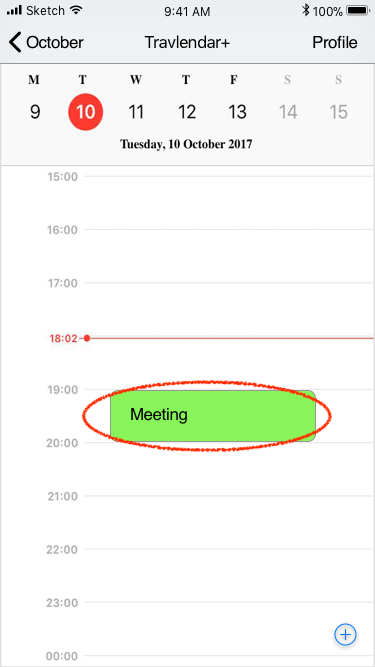
\includegraphics[scale=0.23]{Images/Interface/Directions/1_calendar+meeting}
	\hspace{0.5cm}
	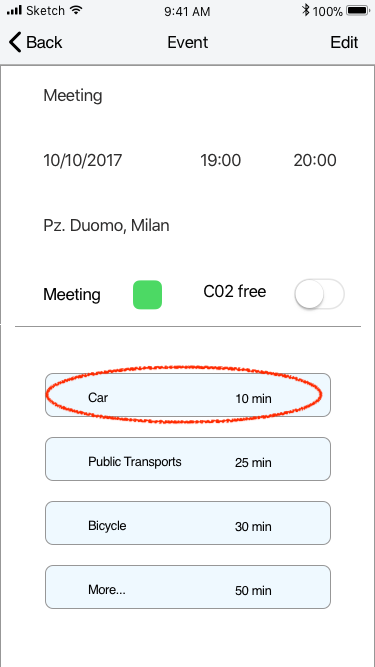
\includegraphics[scale=0.23]{Images/Interface/Directions/2_single_event_view}
	\hspace{0.5cm}
	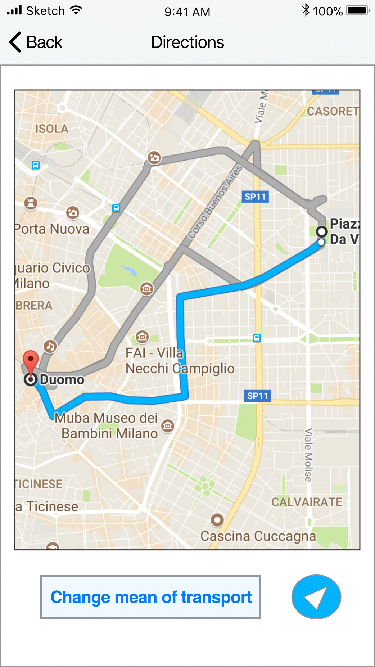
\includegraphics[scale=0.23]{Images/Interface/Directions/3_directions}
	\caption{Directions Sketch}
\end{figure}

\newpage
\mysubsection{Tags}
In this section the user can create tags by tapping on the add button set in the centre-bottom side of the UI.
The user is asked to assign a colour and a name to the tag.
\begin{figure}[H]
	\centering
	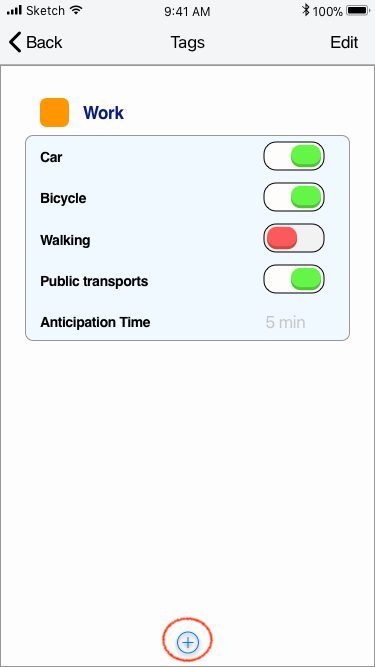
\includegraphics[scale=0.23]{Images/Interface/Tags/1_tags+work_add}
	\hspace{0.5cm}
	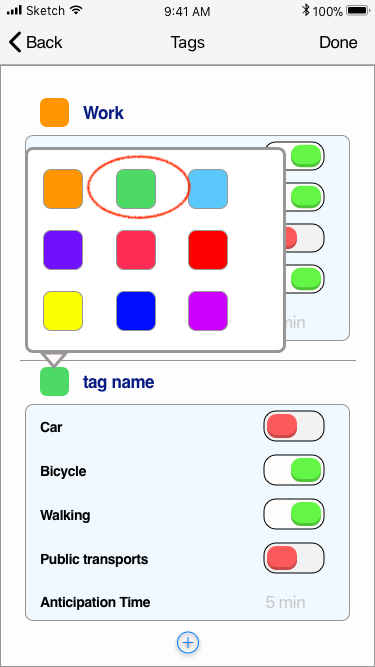
\includegraphics[scale=0.23]{Images/Interface/Tags/2_tags_color}
	\hspace{0.5cm}
	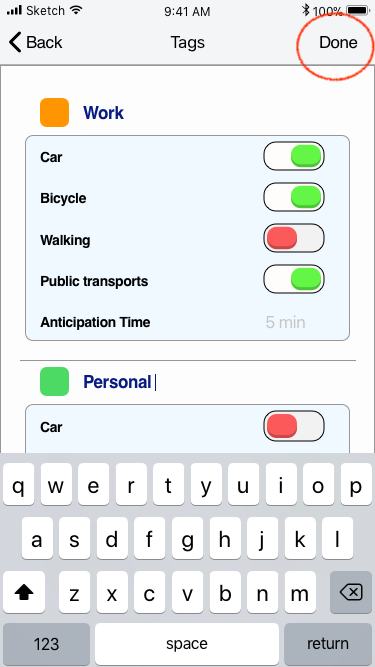
\includegraphics[scale=0.23]{Images/Interface/Tags/3_tag_name}
	\hspace{0.5cm}
	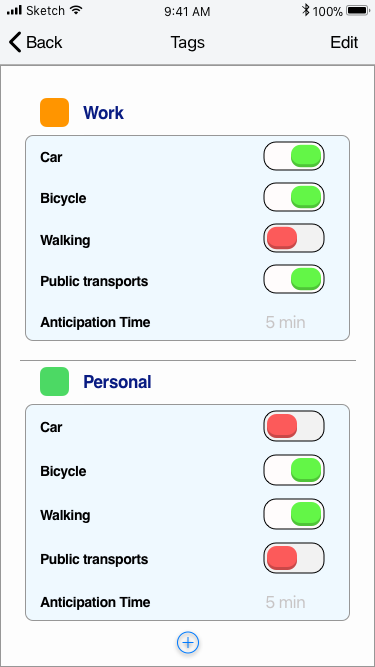
\includegraphics[scale=0.23]{Images/Interface/Tags/4_tags+work+personal}
	\caption{Add Tag Sketches}
\end{figure}
The user can delete one or more tag pressing on the “edit” button and selecting the item he wants to delete.
\begin{figure}[H]
	\centering
	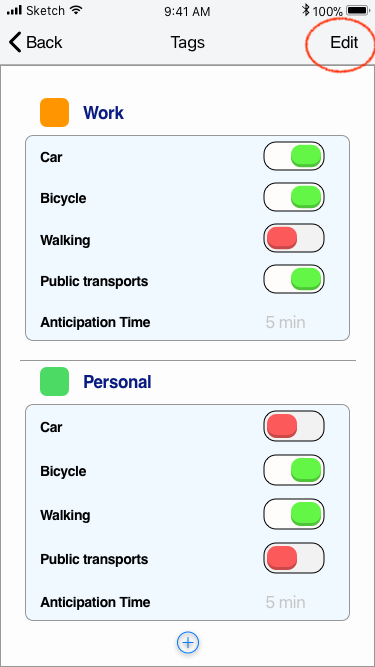
\includegraphics[scale=0.23]{Images/Interface/Tags/5_tags+work+personal-edit}
	\hspace{0.5cm}
	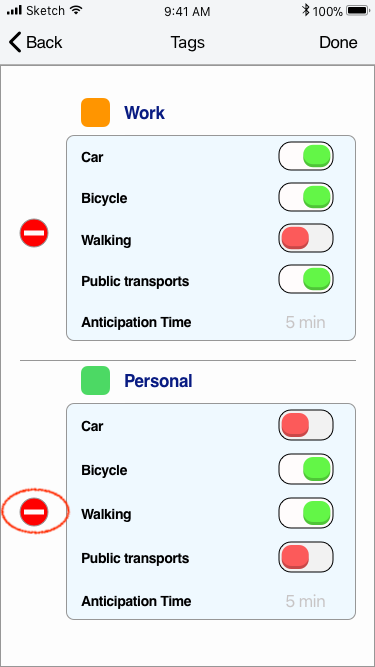
\includegraphics[scale=0.23]{Images/Interface/Tags/6_tags_deletion}
	\hspace{0.5cm}
	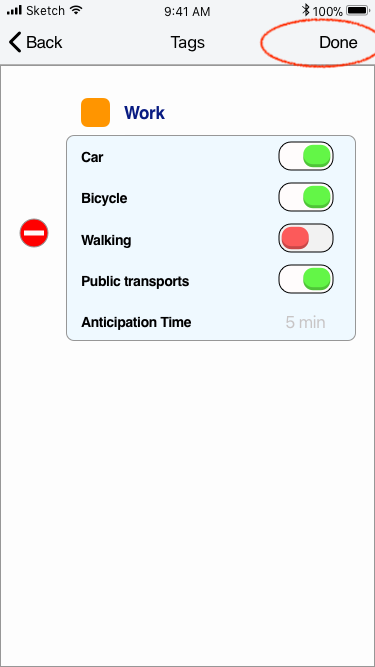
\includegraphics[scale=0.23]{Images/Interface/Tags/7_tags_deletion_2}
	\hspace{0.5cm}
	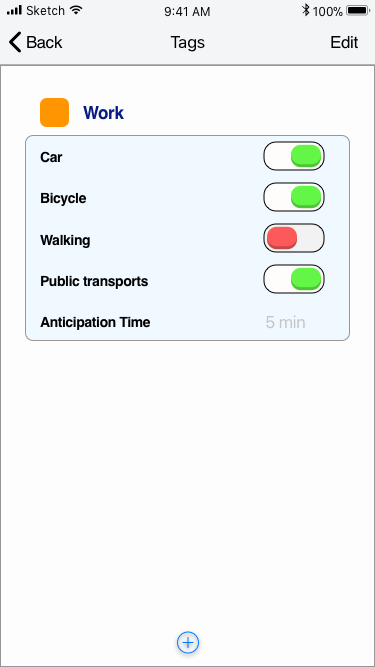
\includegraphics[scale=0.23]{Images/Interface/Tags/8_tags+work}
	\caption{Delete Tag Sketches}
\end{figure}

\newpage
\mysubsection{Trips}
Trips will be suggested if the event is in another town.
\begin{figure}[H]
	\centering
	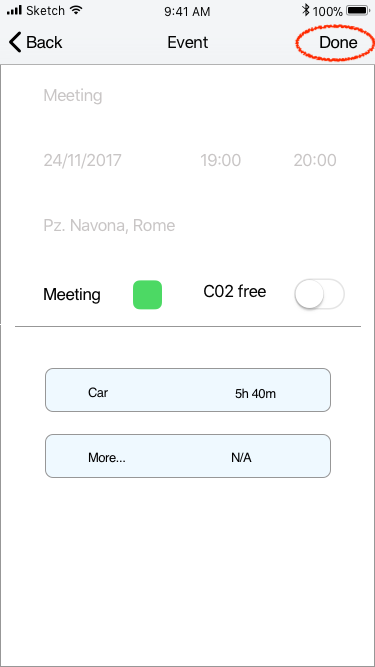
\includegraphics[scale=0.23]{Images/Interface/Trips/1_event_in_rome}
	\hspace{0.5cm}
	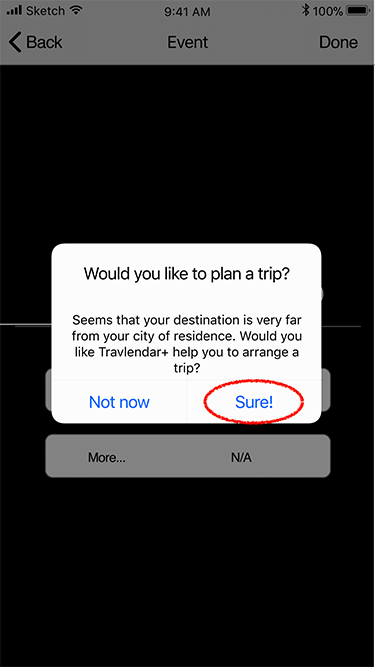
\includegraphics[scale=0.23]{Images/Interface/Trips/2_trip_warning}
	\hspace{0.5cm}
	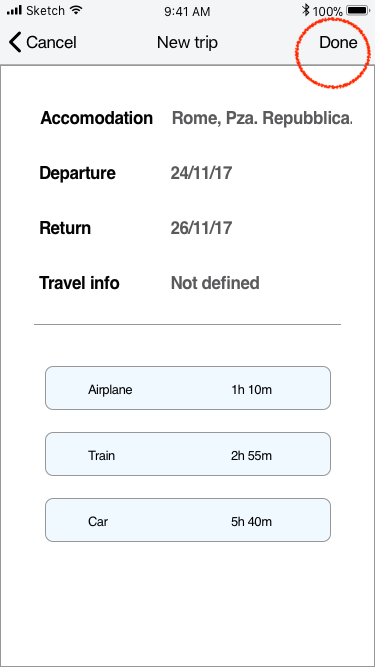
\includegraphics[scale=0.23]{Images/Interface/Trips/3_trip_not_defined}
	\hspace{0.5cm}
	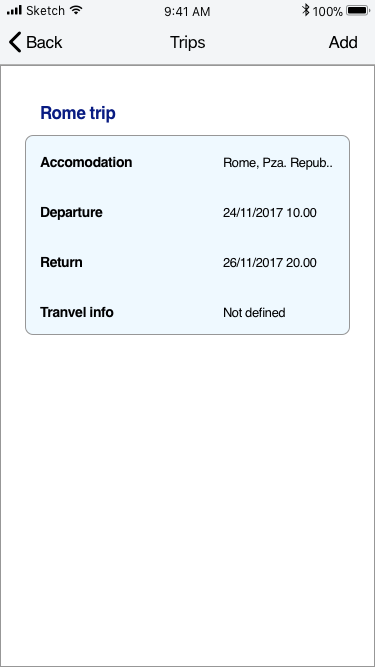
\includegraphics[scale=0.23]{Images/Interface/Trips/4_trips_list}
	\caption{Add Trip Sketches}
\end{figure}
After the creation of a trip, it will be shown also in the profile section.
\begin{figure}[H]
	\centering
	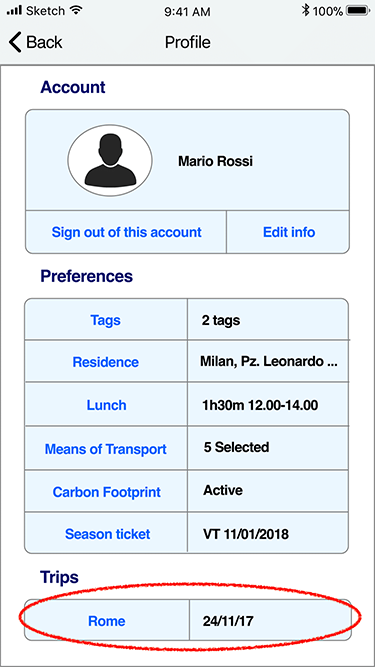
\includegraphics[scale=0.23]{Images/Interface/Trips/5_profile+trips}
	\hspace{0.5cm}
	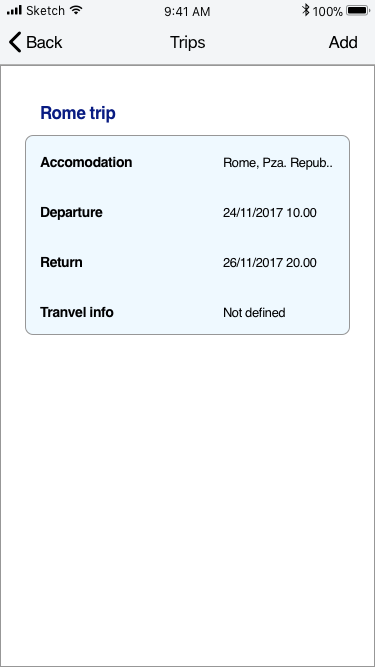
\includegraphics[scale=0.23]{Images/Interface/Trips/6_trip_list}
	\caption{Visualize Trip Sketches}
\end{figure}
The user can insert ticket info by tapping one of the means suggested. By inserting the data, the system will provide some tickets available for the journey. The user will be able to add an existing ticket if he has already bought one (pressing “add”).
\begin{figure}[H]
	\centering
	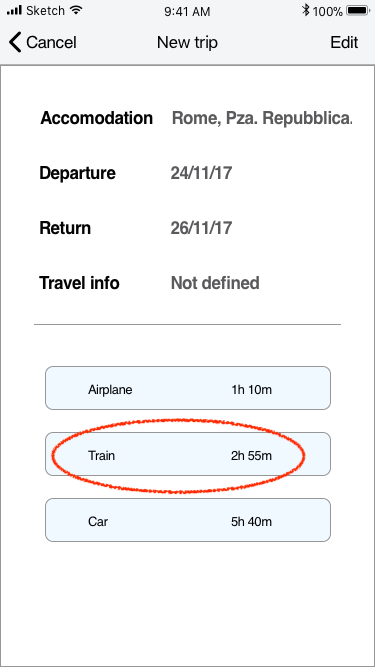
\includegraphics[scale=0.23]{Images/Interface/Trips/7_trip_definition}
	\hspace{0.5cm}
	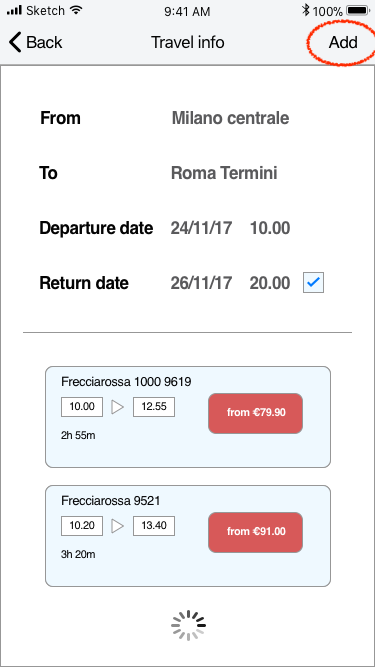
\includegraphics[scale=0.23]{Images/Interface/Trips/8_trip_add_button}
	\hspace{0.5cm}
	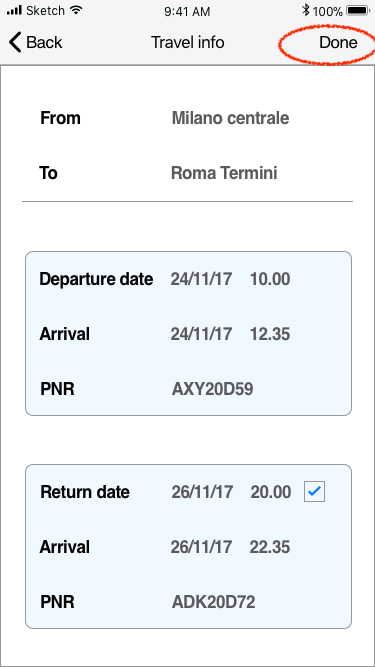
\includegraphics[scale=0.23]{Images/Interface/Trips/9_form}
	\hspace{0.5cm}
	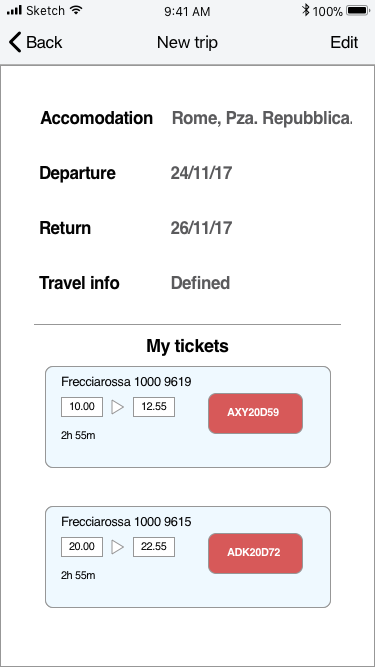
\includegraphics[scale=0.23]{Images/Interface/Trips/10_trip_review}
	\caption{Add Own Tickets Sketches}
\end{figure}
It will be also possible to buy a suggested ticket after being redirected to the service website. If the service does not provide API a manual insertion of the ticket id is required (picture 4 and 5 below).
\begin{figure}[H]
	\centering
	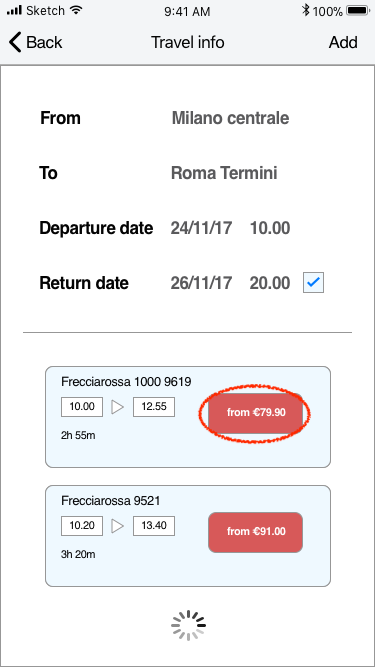
\includegraphics[scale=0.23]{Images/Interface/Trips/11_departure}
	\hspace{0.5cm}
	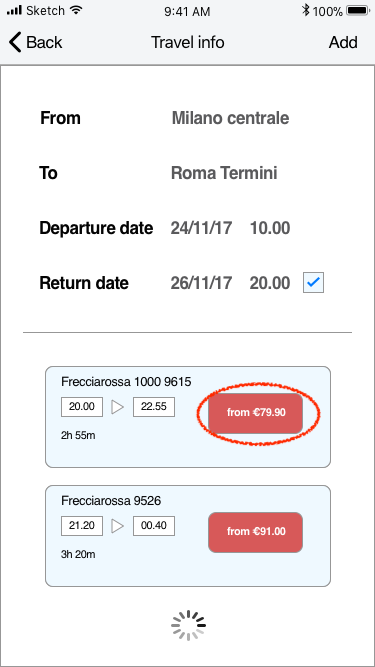
\includegraphics[scale=0.23]{Images/Interface/Trips/12_return}
	\hspace{0.5cm}
	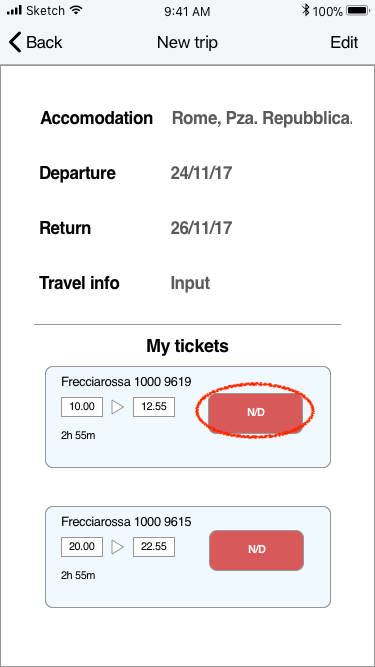
\includegraphics[scale=0.23]{Images/Interface/Trips/13_pnr_to_define}
\end{figure}
\begin{figure}[H]
	\centering
	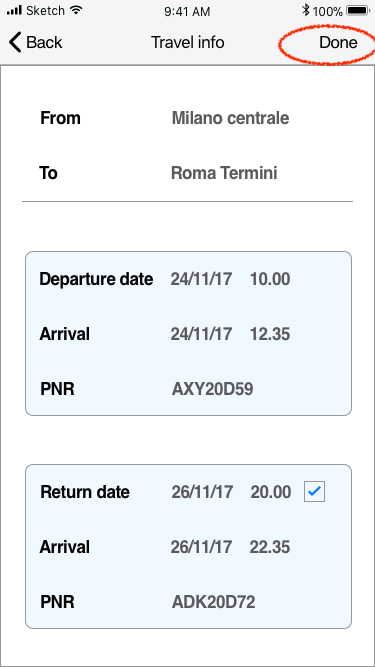
\includegraphics[scale=0.23]{Images/Interface/Trips/14_form}
	\hspace{0.5cm}
	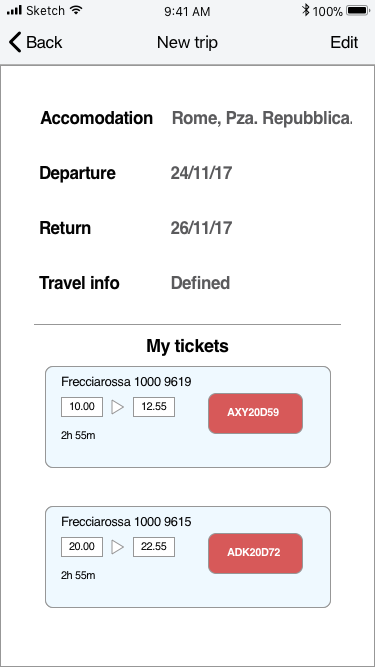
\includegraphics[scale=0.23]{Images/Interface/Trips/15_trip_review}
	\caption{Buy Tickets Sketches}
\end{figure}